\chapter{Measurements}

\definecolor{row-gray}{HTML}{E0E0E0}
\definecolor{row-white}{HTML}{FFFFFF}
\rowcolors{1}{row-white}{row-gray}

The motivation for measuring the compute time for each filter is to help calibrate the filter parameters,
such that frame-rate drops are minimal. In most cases, this measurement is lower than \(33ms\), the timer
set for updating each frame, leading to a mostly constant \(30FPS\). For some filter and parameter
combinations however, this result cannot be achieved, and the user should be advised to run the application
with the frame capture toggled off.

Due to the potential of multi-platform builds, those measurements are also useful in determining system
performance in relation to the processors used for the following computations. Those processors are, in
order of presented measurements, an Intel x86, running at \(2.7GHz\), a Boardcom ARM Cortex-A7, running at
\(900MHz\) on a Raspberry Pi 2B, and a Boardcom ARM Cortex-A72, running at \(1.5GHz\) on a Raspberry Pi 4B
board. \cite{raspi2, raspi4}

In order to compute the measurements, a \(400 \times 400\) image is used, so that it matches the size of
the application viewport, and each parameter is taken as a minimum, median and maximum value. In order to
ensure consistency between consecutive computations, the cache is cleared after each filter instance is
applied.

\section{Box Filter}

The parameters for the box filter are the width and height of the applied kernel. As all parameter
combinations are showcased, several measurements are similar, due to the kernel having the same area,
oriented across a different axis.

\begin{longtable}[H]{|p{4cm}|p{4cm}|>{\raggedleft\arraybackslash}p{4cm}|}
	\hiderowcolors
	\caption{Box Filter Compute time - x86\label{tb:boxFilterX86}}    \\
	\hline
	Kernel size X axis & Kernel size Y axis & Compute time (ms)       \\
	\hline
	\endfirsthead

	\hline
	\multicolumn{3}{|c|}{Continuation of Table \ref{tb:boxFilterX86}} \\
	\hline
	Kernel size X axis & Kernel size Y axis & Compute time (ms)       \\
	\hline
	\endhead

	\hline
	\endfoot

	\hline\hline
	\endlastfoot
	\showrowcolors

	\showrowcolors
	\hline
	3                  & 3                  & 0.15090                 \\
	3                  & 41                 & 0.13247                 \\
	3                  & 79                 & 0.14647                 \\
	41                 & 3                  & 0.16569                 \\
	41                 & 41                 & 0.21468                 \\
	41                 & 79                 & 0.27869                 \\
	79                 & 3                  & 0.19059                 \\
	79                 & 41                 & 0.22782                 \\
	79                 & 79                 & 0.31478                 \\
\end{longtable}

\begin{longtable}[H]{|p{4cm}|p{4cm}|>{\raggedleft\arraybackslash}p{4cm}|}
	\hiderowcolors
	\caption{Box Filter Compute time - Raspberry Pi 2\label{tb:boxFilterRpi2}} \\
	\hline
	Kernel size X axis & Kernel size Y axis & Compute time (ms)                \\
	\hline
	\endfirsthead

	\hline
	\multicolumn{3}{|c|}{Continuation of Table \ref{tb:boxFilterRpi2}}         \\
	\hline
	Kernel size X axis & Kernel size Y axis & Compute time (ms)                \\
	\hline
	\endhead

	\hline
	\endfoot

	\hline\hline
	\endlastfoot
	\showrowcolors

	\hline
	3                  & 3                  & 4.64430                          \\
	3                  & 41                 & 5.01159                          \\
	3                  & 79                 & 5.45388                          \\
	41                 & 3                  & 4.80722                          \\
	41                 & 41                 & 8.62741                          \\
	41                 & 79                 & 9.77371                          \\
	79                 & 3                  & 5.20967                          \\
	79                 & 41                 & 8.78778                          \\
	79                 & 79                 & 9.86720                          \\
\end{longtable}

\begin{longtable}[H]{|p{4cm}|p{4cm}|>{\raggedleft\arraybackslash}p{4cm}|}
	\hiderowcolors
	\caption{Box Filter Compute time - Raspberry Pi 4\label{tb:boxFilterRpi4}} \\
	\hline
	Kernel size X axis & Kernel size Y axis & Compute time (ms)                \\
	\hline
	\endfirsthead

	\hline
	\multicolumn{3}{|c|}{Continuation of Table \ref{tb:boxFilterRpi4}}         \\
	\hline
	Kernel size X axis & Kernel size Y axis & Compute time (ms)                \\
	\hline
	\endhead

	\hline
	\endfoot

	\hline\hline
	\endlastfoot
	\showrowcolors

	\hline
	3                  & 3                  & 1.93976                          \\
	3                  & 41                 & 2.10271                          \\
	3                  & 79                 & 2.46755                          \\
	41                 & 3                  & 1.76251                          \\
	41                 & 41                 & 2.16954                          \\
	41                 & 79                 & 2.61170                          \\
	79                 & 3                  & 2.01735                          \\
	79                 & 41                 & 2.33824                          \\
	79                 & 79                 & 2.58559                          \\
\end{longtable}

As presented, the compute time increases drastically with the kernel size. To be noted, however, is the
significant increase of almost \(100\%\) when going from a \(3\times3\) kernel to a \(41\times41\), opposed
to a less severe \(20\%\) increase between the \(41\times41\) and \(71\times71\) matrices.

\section{Median Filter}

The sole parameter for the median filter is the size of the kernel applied, leading to an increase in area
covered by the computation proportional to the square of the input parameter.

\begin{longtable}[H]{|p{4cm}|>{\raggedleft\arraybackslash}p{4cm}|}
	\hiderowcolors
	\caption{Median Filter Compute time - x86\label{tb:medianFilterX86}} \\
	\hline
	Kernel size & Compute time (ms)                                      \\
	\hline
	\endfirsthead

	\hline
	\multicolumn{2}{|c|}{Continuation of Table \ref{tb:medianFilterX86}} \\
	\hline
	Kernel size & Compute time (ms)                                      \\
	\hline
	\endhead

	\hline
	\endfoot

	\hline\hline
	\endlastfoot
	\showrowcolors

	\hline
	3           & 0.33310                                                \\
	41          & 4.92163                                                \\
	79          & 5.66467                                                \\
\end{longtable}

\begin{longtable}[H]{|p{4cm}|>{\raggedleft\arraybackslash}p{4cm}|}
	\hiderowcolors
	\caption{Median Filter Compute time - Raspberry Pi 2\label{tb:medianFilterRpi2}} \\
	\hline
	Kernel size & Compute time (ms)                                                  \\
	\hline
	\endfirsthead

	\hline
	\multicolumn{2}{|c|}{continuation of table \ref{tb:medianFilterRpi2}}            \\
	\hline
	Kernel size & Compute time (ms)                                                  \\
	\hline
	\endhead

	\hline
	\endfoot

	\hline\hline
	\endlastfoot
	\showrowcolors

	\hline
	3           & 25.03037                                                           \\
	21          & 81.50311                                                           \\
	39          & 137.07168                                                          \\
\end{longtable}

\begin{longtable}[H]{|p{4cm}|>{\raggedleft\arraybackslash}p{4cm}|}
	\hiderowcolors
	\caption{Median Filter Compute time - Raspberry Pi 4\label{tb:medianFilterRpi4}} \\
	\hline
	Kernel size & Compute time (ms)                                                 \\
	\hline
	\endfirsthead

	\hline
	\multicolumn{2}{|c|}{Continuation of Table \ref{tb:medianFilterRpi4}}           \\
	\hline
	Kernel size & Compute time (ms)                                                 \\
	\hline
	\endhead

	\hline
	\endfoot

	\hline\hline
	\endlastfoot
	\showrowcolors

	\hline
	3           & 1.71151                                                           \\
	21          & 39.11374                                                          \\
	39          & 39.66373                                                          \\
\end{longtable}

Due to the significant increase in the amount of computations due to the larger coverage, the filter
performance is greatly affected by high values for the kernel size. Because of this measurement, the
maximum value for the size parameter has been severely reduced for the final version of the application.

\section{Erode Filter}

Similar to the median filter, the erode computation also takes the kernel size as the only input. The
overall amount of operations is, however, drastically lower, due to the need to compute the minimum value
withing the kernel area, as opposed to the median.

\begin{longtable}[H]{|p{4cm}|>{\raggedleft\arraybackslash}p{4cm}|}
	\hiderowcolors
	\caption{Erode Filter Compute time - x86\label{tb:erodeFilterX86}}  \\
	\hline
	Kernel size & Compute time (ms)                                     \\
	\hline
	\endfirsthead

	\hline
	\multicolumn{2}{|c|}{Continuation of Table \ref{tb:erodeFilterX86}} \\
	\hline
	Kernel size & Compute time (ms)                                     \\
	\hline
	\endhead

	\hline
	\endfoot

	\hline\hline
	\endlastfoot
	\showrowcolors

	\hline
	3           & 0.07016                                               \\
	25          & 0.16817                                               \\
	47          & 0.29865                                               \\
\end{longtable}

\begin{longtable}[H]{|p{4cm}|>{\raggedleft\arraybackslash}p{4cm}|}
	\hiderowcolors
	\caption{Erode Filter Compute time - Raspberry Pi 2\label{tb:erodeFilterRpi2}} \\
	\hline
	Kernel size & Compute time (ms)                                                \\
	\hline
	\endfirsthead

	\hline
	\multicolumn{2}{|c|}{Continuation of Table \ref{tb:erodeFilterRpi2}}           \\
	\hline
	Kernel size & Compute time (ms)                                                \\
	\hline
	\endhead

	\hline
	\endfoot

	\hline\hline
	\endlastfoot
	\showrowcolors

	\hline
	3           & 6.79081                                                          \\
	25          & 40.13298                                                         \\
	47          & 75.35150                                                         \\
\end{longtable}

\begin{longtable}[H]{|p{4cm}|>{\raggedleft\arraybackslash}p{4cm}|}
	\hiderowcolors
	\caption{Erode Filter Compute time - Raspberry Pi 4\label{tb:erodeFilterRpi4}} \\
	\hline
	Kernel size & Compute time (ms)                                                \\
	\hline
	\endfirsthead

	\hline
	\multicolumn{2}{|c|}{Continuation of Table \ref{tb:erodeFilterRpi4}}           \\
	\hline
	Kernel size & Compute time (ms)                                                \\
	\hline
	\endhead

	\hline
	\endfoot

	\hline\hline
	\endlastfoot
	\showrowcolors

	\hline
	3           & 0.40999                                                          \\
	25          & 1.76110                                                          \\
	47          & 3.29456                                                          \\
\end{longtable}

As expected, the overall compute time is significantly lower than in the case of the median filter. It can
also be observed that, for the Raspberry Pi 2, the operation took an order of magnitude longer to complete.

\section{Dilate Filter}

The dilate filter, providing the exact opposite functionality to the erode filter, computing the maximum
value with the structuring element instead of the minimum, also takes in as parameter the size of that
specific structuring element.

\begin{longtable}[H]{|p{4cm}|>{\raggedleft\arraybackslash}p{4cm}|}
	\hiderowcolors
	\caption{Dilate Filter Compute time - x86\label{tb:dilateFilterX86}} \\
	\hline
	Kernel size & Compute time (ms)                                      \\
	\hline
	\endfirsthead

	\hline
	\multicolumn{2}{|c|}{Continuation of Table \ref{tb:dilateFilterX86}} \\
	\hline
	Kernel size & Compute time (ms)                                      \\
	\hline
	\endhead

	\hline
	\endfoot

	\hline\hline
	\endlastfoot
	\showrowcolors

	\hline
	3           & 0.10545                                                \\
	25          & 0.16417                                                \\
	47          & 0.28653                                                \\
\end{longtable}

\begin{longtable}[H]{|p{4cm}|>{\raggedleft\arraybackslash}p{4cm}|}
	\hiderowcolors
	\caption{Dilate Filter Compute time - Raspberry Pi 2\label{tb:dilateFilterRpi2}} \\
	\hline
	Kernel size & Compute time (ms)                                                  \\
	\hline
	\endfirsthead

	\hline
	\multicolumn{2}{|c|}{Continuation of Table \ref{tb:dilateFilterRpi2}}            \\
	\hline
	Kernel size & Compute time (ms)                                                  \\
	\hline
	\endhead

	\hline
	\endfoot

	\hline\hline
	\endlastfoot
	\showrowcolors

	\hline
	3           & 6.92024                                                            \\
	25          & 40.20611                                                           \\
	47          & 75.51301                                                           \\
\end{longtable}

\begin{longtable}[H]{|p{4cm}|>{\raggedleft\arraybackslash}p{4cm}|}
	\hiderowcolors
	\caption{Dilate Filter Compute time - Raspberry Pi 4\label{tb:dilateFilterRpi4}} \\
	\hline
	Kernel size & Compute time (ms)                                                  \\
	\hline
	\endfirsthead

	\hline
	\multicolumn{2}{|c|}{Continuation of Table \ref{tb:dilateFilterRpi4}}            \\
	\hline
	Kernel size & Compute time (ms)                                                  \\
	\hline
	\endhead

	\hline
	\endfoot

	\hline\hline
	\endlastfoot
	\showrowcolors

	\hline
	3           & 0.57249                                                            \\
	25          & 1.86577                                                            \\
	47          & 3.44228                                                            \\
\end{longtable}

Also due to being essentially identical, the compute time for both the erode and dilate filters are within
a \(100-th\) of a millisecond apart.

\section{Gaussian Filter}

The Gaussian filter, in addition to the kernel size, is parameterized by the \(\sigma\) value for each of the
axes. Those control the spread of the Gaussian distribution under the kernel.

\begin{longtable}[H]{|p{3cm}|p{3cm}|p{3cm}|>{\raggedleft\arraybackslash}p{3cm}|}
	\hiderowcolors
	\caption{Gaussian Filter Compute time - x86\label{tb:gaussianFilterX86}}   \\
	\hline
	Kernel size & Sigma value on X axis & Sigma value on Y axis & Compute time \\
	\hline
	\endfirsthead

	\hline
	\multicolumn{4}{|c|}{Continuation of Table \ref{tb:gaussianFilterX86}}     \\
	\hline
	Kernel size & Sigma value on X axis & Sigma value on Y axis & Compute time \\
	\hline
	\endhead

	\hline
	\endfoot

	\hline\hline
	\endlastfoot
	\showrowcolors

	\hline
	3           & 1                     & 1                     & 0.98044      \\
	3           & 1                     & 51                    & 0.16341      \\
	3           & 1                     & 101                   & 0.16001      \\
	3           & 51                    & 1                     & 0.15809      \\
	3           & 51                    & 51                    & 0.15840      \\
	3           & 51                    & 101                   & 0.15436      \\
	3           & 101                   & 1                     & 0.15957      \\
	3           & 101                   & 51                    & 0.15555      \\
	3           & 101                   & 101                   & 0.19613      \\
	41          & 1                     & 1                     & 0.67182      \\
	41          & 1                     & 51                    & 0.93343      \\
	41          & 1                     & 101                   & 0.61505      \\
	41          & 51                    & 1                     & 3.31605      \\
	41          & 51                    & 51                    & 3.21340      \\
	41          & 51                    & 101                   & 3.23505      \\
	41          & 101                   & 1                     & 3.23909      \\
	41          & 101                   & 51                    & 3.24750      \\
	41          & 101                   & 101                   & 3.36258      \\
	79          & 1                     & 1                     & 1.03642      \\
	79          & 1                     & 51                    & 1.00481      \\
	79          & 1                     & 101                   & 1.00744      \\
	79          & 51                    & 1                     & 13.19533     \\
	79          & 51                    & 51                    & 13.41555     \\
	79          & 51                    & 101                   & 13.44934     \\
	79          & 101                   & 1                     & 13.30223     \\
	79          & 101                   & 51                    & 14.28438     \\
	79          & 101                   & 101                   & 13.39821     \\
\end{longtable}

\begin{longtable}[H]{|p{3cm}|p{3cm}|p{3cm}|>{\raggedleft\arraybackslash}p{3cm}|}
	\hiderowcolors
	\caption{Gaussian Filter Compute time - Raspberry Pi 2\label{tb:gaussianFilterRpi2}} \\
	\hline
	Kernel size & Sigma value on X axis & Sigma value on Y axis & Compute time (ms)      \\
	\hline
	\endfirsthead

	\hline
	\multicolumn{4}{|c|}{Continuation of Table \ref{tb:gaussianFilterRpi2}}              \\
	\hline
	Kernel size & Sigma value on X axis & Sigma value on Y axis & Compute time (ms)      \\
	\hline
	\endhead

	\hline
	\endfoot

	\hline\hline
	\endlastfoot
	\showrowcolors

	\hline
	3           & 1                     & 1                     & 4.94128                \\
	3           & 1                     & 51                    & 4.55691                \\
	3           & 1                     & 101                   & 5.09066                \\
	3           & 51                    & 1                     & 4.50535                \\
	3           & 51                    & 51                    & 4.71201                \\
	3           & 51                    & 101                   & 4.65712                \\
	3           & 101                   & 1                     & 4.54670                \\
	3           & 101                   & 51                    & 4.38873                \\
	3           & 101                   & 101                   & 4.45941                \\
	41          & 1                     & 1                     & 59.18977               \\
	41          & 1                     & 51                    & 59.24013               \\
	41          & 1                     & 101                   & 59.22039               \\
	41          & 51                    & 1                     & 59.22805               \\
	41          & 51                    & 51                    & 59.30581               \\
	41          & 51                    & 101                   & 59.23857               \\
	41          & 101                   & 1                     & 59.22654               \\
	41          & 101                   & 51                    & 59.64451               \\
	41          & 101                   & 101                   & 59.27930               \\
	79          & 1                     & 1                     & 113.47222              \\
	79          & 1                     & 51                    & 112.74847              \\
	79          & 1                     & 101                   & 112.62124              \\
	79          & 51                    & 1                     & 112.49009              \\
	79          & 51                    & 51                    & 112.85811              \\
	79          & 51                    & 101                   & 112.80249              \\
	79          & 101                   & 1                     & 112.70978              \\
	79          & 101                   & 51                    & 112.88249              \\
	79          & 101                   & 101                   & 112.77332              \\
\end{longtable}

\begin{longtable}[H]{|p{3cm}|p{3cm}|p{3cm}|>{\raggedleft\arraybackslash}p{3cm}|}
	\hiderowcolors
	\caption{Gaussian Filter Compute time - Raspberry Pi 4\label{tb:gaussianFilterRpi4}} \\
	\hline
	Kernel size & Sigma value on X axis & Sigma value on Y axis & Compute time (ms)      \\
	\hline
	\endfirsthead

	\hline
	\multicolumn{4}{|c|}{Continuation of Table \ref{tb:gaussianFilterRpi4}}              \\
	\hline
	Kernel size & Sigma value on X axis & Sigma value on Y axis & Compute time (ms)      \\
	\hline
	\endhead

	\hline
	\endfoot

	\hline\hline
	\endlastfoot
	\showrowcolors

	\hline
	3           & 1                     & 1                     & 14.60446               \\
	3           & 1                     & 51                    & 1.46411                \\
	3           & 1                     & 101                   & 0.97422                \\
	3           & 51                    & 1                     & 1.00395                \\
	3           & 51                    & 51                    & 0.98398                \\
	3           & 51                    & 101                   & 0.95282                \\
	3           & 101                   & 1                     & 1.02545                \\
	3           & 101                   & 51                    & 0.93567                \\
	3           & 101                   & 101                   & 0.91604                \\
	41          & 1                     & 1                     & 4.81236                \\
	41          & 1                     & 51                    & 4.70063                \\
	41          & 1                     & 101                   & 4.81916                \\
	41          & 51                    & 1                     & 13.24067               \\
	41          & 51                    & 51                    & 13.16267               \\
	41          & 51                    & 101                   & 13.19019               \\
	41          & 101                   & 1                     & 13.14162               \\
	41          & 101                   & 51                    & 23.38182               \\
	41          & 101                   & 101                   & 13.12504               \\
	79          & 1                     & 1                     & 8.65297                \\
	79          & 1                     & 51                    & 8.83360                \\
	79          & 1                     & 101                   & 8.55154                \\
	79          & 51                    & 1                     & 48.49909               \\
	79          & 51                    & 51                    & 48.12615               \\
	79          & 51                    & 101                   & 48.34737               \\
	79          & 101                   & 1                     & 48.23959               \\
	79          & 101                   & 51                    & 49.48103               \\
	79          & 101                   & 101                   & 48.24783               \\
\end{longtable}

Due to the nature of the filter, an increase in \(\sigma\) value leads to an increase in the compute time.
This is due to the Gaussian distribution accounting for more of the surrounding neighborhood, leading to
more expensive computations.

\section{Bilateral Correction}

The parameters for the bilateral correction are the kernel size, \(\sigma_{color}\) and \(\sigma_{space}\)
values. Both \(\sigma\) values denote how much of the surrounding neighborhood affects the current pixel
value, both in terms of intensity, as well as in color.

\begin{longtable}[H]{|p{3cm}|p{3cm}|p{3cm}|>{\raggedleft\arraybackslash}p{3cm}|}
	\hiderowcolors
	\caption{Bilateral Correction Compute time - x86\label{tb:bilateralFilterX86}} \\
	\hline
	Kernel size & Sigma color value & Sigma space value & Compute time (ms)        \\
	\hline
	\endfirsthead

	\hline
	\multicolumn{4}{|c|}{Continuation of Table \ref{tb:bilateralFilterX86}}        \\
	\hline
	Kernel size & Sigma color value & Sigma space value & Compute time (ms)        \\
	\hline
	\endhead

	\hline
	\endfoot

	\hline\hline
	\endlastfoot
	\showrowcolors

	\hline
	3           & 1                 & 1                 & 0.46384                  \\
	3           & 1                 & 51                & 0.34726                  \\
	3           & 1                 & 101               & 0.33460                  \\
	3           & 51                & 1                 & 0.33997                  \\
	3           & 51                & 51                & 0.34069                  \\
	3           & 51                & 101               & 0.33945                  \\
	3           & 101               & 1                 & 0.34287                  \\
	3           & 101               & 51                & 0.34193                  \\
	3           & 101               & 101               & 0.34163                  \\
	7           & 1                 & 1                 & 5.99946                  \\
	7           & 1                 & 51                & 5.76259                  \\
	7           & 1                 & 101               & 6.48361                  \\
	7           & 51                & 1                 & 6.00622                  \\
	7           & 51                & 51                & 5.87350                  \\
	7           & 51                & 101               & 6.45825                  \\
	7           & 101               & 1                 & 6.16447                  \\
	7           & 101               & 51                & 6.27419                  \\
	7           & 101               & 101               & 6.00010                  \\
	11          & 1                 & 1                 & 14.67617                 \\
	11          & 1                 & 51                & 15.17843                 \\
	11          & 1                 & 101               & 15.32325                 \\
	11          & 51                & 1                 & 15.34834                 \\
	11          & 51                & 51                & 14.63266                 \\
	11          & 51                & 101               & 15.48984                 \\
	11          & 101               & 1                 & 15.55351                 \\
	11          & 101               & 51                & 14.83601                 \\
	11          & 101               & 101               & 14.66591                 \\
\end{longtable}

\begin{longtable}[H]{|p{3cm}|p{3cm}|p{3cm}|>{\raggedleft\arraybackslash}p{3cm}|}
	\hiderowcolors
	\caption{Bilateral Correction Compute time - Raspberry Pi 2\label{tb:bilateralFilterRpi2}} \\
	\hline
	Kernel size & Sigma color value & Sigma space value & Compute time (ms)                    \\
	\hline
	\endfirsthead

	\hline
	\multicolumn{4}{|c|}{Continuation of Table \ref{tb:bilateralFilterRpi2}}                   \\
	\hline
	Kernel size & Sigma color value & Sigma space value & Compute time (ms)                    \\
	\hline
	\endhead

	\hline
	\endfoot

	\hline\hline
	\endlastfoot
	\showrowcolors

	\hline
	3           & 1                 & 1                 & 15.93234                             \\
	3           & 1                 & 51                & 15.52202                             \\
	3           & 1                 & 101               & 15.47854                             \\
	3           & 51                & 1                 & 15.66333                             \\
	3           & 51                & 51                & 15.59869                             \\
	3           & 51                & 101               & 15.61885                             \\
	3           & 101               & 1                 & 15.64760                             \\
	3           & 101               & 51                & 15.58343                             \\
	3           & 101               & 101               & 15.55374                             \\
	7           & 1                 & 1                 & 67.42861                             \\
	7           & 1                 & 51                & 67.42059                             \\
	7           & 1                 & 101               & 67.24694                             \\
	7           & 51                & 1                 & 67.40163                             \\
	7           & 51                & 51                & 67.46871                             \\
	7           & 51                & 101               & 67.50246                             \\
	7           & 101               & 1                 & 67.42184                             \\
	7           & 101               & 51                & 67.49257                             \\
	7           & 101               & 101               & 67.39246                             \\
	11          & 1                 & 1                 & 179.86232                            \\
	11          & 1                 & 51                & 179.80378                            \\
	11          & 1                 & 101               & 179.78175                            \\
	11          & 51                & 1                 & 179.96326                            \\
	11          & 51                & 51                & 179.82425                            \\
	11          & 51                & 101               & 179.85378                            \\
	11          & 101               & 1                 & 179.92159                            \\
	11          & 101               & 51                & 180.05618                            \\
	11          & 101               & 101               & 179.93613                            \\
\end{longtable}

\begin{longtable}[H]{|p{3cm}|p{3cm}|p{3cm}|>{\raggedleft\arraybackslash}p{3cm}|}
	\hiderowcolors
	\caption{Bilateral Correction Compute time - Raspberry Pi 4\label{tb:bilateralFilterRpi4}} \\
	\hline
	Kernel size & Sigma color value & Sigma space value & Compute time (ms)                    \\
	\hline
	\endfirsthead

	\hline
	\multicolumn{4}{|c|}{Continuation of Table \ref{tb:bilateralFilterRpi4}}                   \\
	\hline
	Kernel size & Sigma color value & Sigma space value & Compute time (ms)                    \\
	\hline
	\endhead

	\hline
	\endfoot

	\hline\hline
	\endlastfoot
	\showrowcolors

	\hline
	3           & 1                 & 1                 & 5.58308                              \\
	3           & 1                 & 51                & 5.09406                              \\
	3           & 1                 & 101               & 5.17097                              \\
	3           & 51                & 1                 & 5.31986                              \\
	3           & 51                & 51                & 5.36273                              \\
	3           & 51                & 101               & 5.28336                              \\
	3           & 101               & 1                 & 5.19588                              \\
	3           & 101               & 51                & 5.17456                              \\
	3           & 101               & 101               & 5.16075                              \\
	7           & 1                 & 1                 & 23.15716                             \\
	7           & 1                 & 51                & 23.09940                             \\
	7           & 1                 & 101               & 23.11199                             \\
	7           & 51                & 1                 & 23.08756                             \\
	7           & 51                & 51                & 23.14056                             \\
	7           & 51                & 101               & 23.07794                             \\
	7           & 101               & 1                 & 23.10047                             \\
	7           & 101               & 51                & 23.26132                             \\
	7           & 101               & 101               & 23.23467                             \\
	11          & 1                 & 1                 & 62.35211                             \\
	11          & 1                 & 51                & 61.73884                             \\
	11          & 1                 & 101               & 61.67917                             \\
	11          & 51                & 1                 & 61.53942                             \\
	11          & 51                & 51                & 61.58005                             \\
	11          & 51                & 101               & 61.59607                             \\
	11          & 101               & 1                 & 61.62008                             \\
	11          & 101               & 51                & 61.56597                             \\
	11          & 101               & 101               & 61.53334                             \\
\end{longtable}

The kernel size is the most relevant parameter, as it denotes the amount of surrounding pixels that need to
be accounted for when performing the correction. Because of the specifically high compute time and the
preference of using this filter in conjunction with an edge detection convolution, it is recommended, for
best results, that this filter be used with the frame capture toggled off.

\section{Sobel Filter}

Used for edge detection, the Sobel filter computes frequency derivatives using the extended Sobel operators.
The order of the derivative is specified with respect to each axis, and the kernel size denotes the breadth
of the operator. Because the edge angle can also be computed, a boolean is also provided to the filter
wrapper in order to toggle this functionality.

\begin{longtable}[H]{|p{2cm}|p{2cm}|p{2cm}|p{2cm}|>{\raggedleft\arraybackslash}p{2cm}|}
	\hiderowcolors
	\caption{Sobel Filter Compute time - x86\label{tb:sobelFilterX86}}                           \\
	\hline
	Display direction & Kernel size & Derivative on X axis & Derivative on Y axis & Compute time \\
	\hline
	\endfirsthead

	\hline
	\multicolumn{5}{|c|}{Continuation of Table \ref{tb:sobelFilterX86}}                          \\
	\hline
	Display direction & Kernel size & Derivative on X axis & Derivative on Y axis & Compute time \\
	\hline
	\endhead

	\hline
	\endfoot

	\hline\hline
	\endlastfoot
	\showrowcolors

	\hline
	0                 & 3           & 1                    & 1                    & 1.14748      \\
	0                 & 3           & 1                    & 2                    & 0.88707      \\
	0                 & 3           & 1                    & 3                    & 0.90265      \\
	0                 & 3           & 2                    & 1                    & 0.94404      \\
	0                 & 3           & 2                    & 2                    & 0.83073      \\
	0                 & 3           & 2                    & 3                    & 0.87637      \\
	0                 & 3           & 3                    & 1                    & 0.80348      \\
	0                 & 3           & 3                    & 2                    & 0.81637      \\
	0                 & 3           & 3                    & 3                    & 0.84181      \\
	0                 & 5           & 1                    & 1                    & 1.05125      \\
	0                 & 5           & 1                    & 2                    & 1.02821      \\
	0                 & 5           & 1                    & 3                    & 0.93255      \\
	0                 & 5           & 2                    & 1                    & 0.94318      \\
	0                 & 5           & 2                    & 2                    & 1.05751      \\
	0                 & 5           & 2                    & 3                    & 1.01842      \\
	0                 & 5           & 3                    & 1                    & 0.95572      \\
	0                 & 5           & 3                    & 2                    & 0.97114      \\
	0                 & 5           & 3                    & 3                    & 0.95624      \\
	0                 & 7           & 1                    & 1                    & 1.11434      \\
	0                 & 7           & 1                    & 2                    & 1.12400      \\
	0                 & 7           & 1                    & 3                    & 1.11073      \\
	0                 & 7           & 2                    & 1                    & 1.11029      \\
	0                 & 7           & 2                    & 2                    & 1.12417      \\
	0                 & 7           & 2                    & 3                    & 1.09196      \\
	0                 & 7           & 3                    & 1                    & 1.13244      \\
	0                 & 7           & 3                    & 2                    & 1.11799      \\
	0                 & 7           & 3                    & 3                    & 1.17622      \\
	1                 & 3           & 1                    & 1                    & 6.60175      \\
	1                 & 3           & 1                    & 2                    & 7.14455      \\
	1                 & 3           & 1                    & 3                    & 7.36451      \\
	1                 & 3           & 2                    & 1                    & 6.92685      \\
	1                 & 3           & 2                    & 2                    & 7.00550      \\
	1                 & 3           & 2                    & 3                    & 6.96992      \\
	1                 & 3           & 3                    & 1                    & 6.84147      \\
	1                 & 3           & 3                    & 2                    & 7.29929      \\
	1                 & 3           & 3                    & 3                    & 7.02214      \\
	1                 & 5           & 1                    & 1                    & 10.83666     \\
	1                 & 5           & 1                    & 2                    & 6.85438      \\
	1                 & 5           & 1                    & 3                    & 7.01054      \\
	1                 & 5           & 2                    & 1                    & 7.15676      \\
	1                 & 5           & 2                    & 2                    & 6.87764      \\
	1                 & 5           & 2                    & 3                    & 7.82843      \\
	1                 & 5           & 3                    & 1                    & 7.42942      \\
	1                 & 5           & 3                    & 2                    & 8.17122      \\
	1                 & 5           & 3                    & 3                    & 6.98405      \\
	1                 & 7           & 1                    & 1                    & 6.94443      \\
	1                 & 7           & 1                    & 2                    & 6.95331      \\
	1                 & 7           & 1                    & 3                    & 6.84935      \\
	1                 & 7           & 2                    & 1                    & 7.06645      \\
	1                 & 7           & 2                    & 2                    & 7.10490      \\
	1                 & 7           & 2                    & 3                    & 6.98955      \\
	1                 & 7           & 3                    & 1                    & 6.98345      \\
	1                 & 7           & 3                    & 2                    & 7.03998      \\
	1                 & 7           & 3                    & 3                    & 7.03961      \\
\end{longtable}

\begin{longtable}[H]{|p{2cm}|p{2cm}|p{2cm}|p{2cm}|>{\raggedleft\arraybackslash}p{2cm}|}
	\hiderowcolors
	\caption{Sobel Filter Compute time - Raspberry Pi 2\label{tb:sobelFilterRpi2}}               \\
	\hline
	Display direction & Kernel size & Derivative on X axis & Derivative on Y axis & Compute time \\
	\hline
	\endfirsthead

	\hline
	\multicolumn{5}{|c|}{Continuation of Table \ref{tb:sobelFilterRpi2}}                         \\
	\hline
	Display direction & Kernel size & Derivative on X axis & Derivative on Y axis & Compute time \\
	\hline
	\endhead

	\hline
	\endfoot

	\hline\hline
	\endlastfoot
	\showrowcolors

	\hline
	0                 & 3           & 1                    & 1                    & 14.27584     \\
	0                 & 3           & 1                    & 2                    & 13.63375     \\
	0                 & 3           & 1                    & 3                    & 13.68297     \\
	0                 & 3           & 2                    & 1                    & 13.32266     \\
	0                 & 3           & 2                    & 2                    & 13.58235     \\
	0                 & 3           & 2                    & 3                    & 13.65651     \\
	0                 & 3           & 3                    & 1                    & 13.32678     \\
	0                 & 3           & 3                    & 2                    & 13.59990     \\
	0                 & 3           & 3                    & 3                    & 13.80042     \\
	0                 & 5           & 1                    & 1                    & 16.48859     \\
	0                 & 5           & 1                    & 2                    & 16.67140     \\
	0                 & 5           & 1                    & 3                    & 16.40244     \\
	0                 & 5           & 2                    & 1                    & 16.35489     \\
	0                 & 5           & 2                    & 2                    & 16.64296     \\
	0                 & 5           & 2                    & 3                    & 16.27989     \\
	0                 & 5           & 3                    & 1                    & 16.34734     \\
	0                 & 5           & 3                    & 2                    & 16.57078     \\
	0                 & 5           & 3                    & 3                    & 16.35776     \\
	0                 & 7           & 1                    & 1                    & 19.44519     \\
	0                 & 7           & 1                    & 2                    & 19.87238     \\
	0                 & 7           & 1                    & 3                    & 19.47681     \\
	0                 & 7           & 2                    & 1                    & 19.54103     \\
	0                 & 7           & 2                    & 2                    & 19.82879     \\
	0                 & 7           & 2                    & 3                    & 19.52228     \\
	0                 & 7           & 3                    & 1                    & 19.53358     \\
	0                 & 7           & 3                    & 2                    & 19.80488     \\
	0                 & 7           & 3                    & 3                    & 19.42452     \\
	1                 & 3           & 1                    & 1                    & 108.07677    \\
	1                 & 3           & 1                    & 2                    & 107.60281    \\
	1                 & 3           & 1                    & 3                    & 106.54724    \\
	1                 & 3           & 2                    & 1                    & 106.45162    \\
	1                 & 3           & 2                    & 2                    & 106.02386    \\
	1                 & 3           & 2                    & 3                    & 106.13204    \\
	1                 & 3           & 3                    & 1                    & 106.41277    \\
	1                 & 3           & 3                    & 2                    & 106.05042    \\
	1                 & 3           & 3                    & 3                    & 105.99985    \\
	1                 & 5           & 1                    & 1                    & 110.69478    \\
	1                 & 5           & 1                    & 2                    & 109.66901    \\
	1                 & 5           & 1                    & 3                    & 110.52531    \\
	1                 & 5           & 2                    & 1                    & 111.03442    \\
	1                 & 5           & 2                    & 2                    & 110.22822    \\
	1                 & 5           & 2                    & 3                    & 111.04176    \\
	1                 & 5           & 3                    & 1                    & 110.71000    \\
	1                 & 5           & 3                    & 2                    & 109.88083    \\
	1                 & 5           & 3                    & 3                    & 110.57734    \\
	1                 & 7           & 1                    & 1                    & 113.26275    \\
	1                 & 7           & 1                    & 2                    & 110.87484    \\
	1                 & 7           & 1                    & 3                    & 111.15203    \\
	1                 & 7           & 2                    & 1                    & 112.36124    \\
	1                 & 7           & 2                    & 2                    & 111.55109    \\
	1                 & 7           & 2                    & 3                    & 112.08728    \\
	1                 & 7           & 3                    & 1                    & 112.30270    \\
	1                 & 7           & 3                    & 2                    & 111.62119    \\
	1                 & 7           & 3                    & 3                    & 112.13322    \\
\end{longtable}

\begin{longtable}[H]{|p{2cm}|p{2cm}|p{2cm}|p{2cm}|>{\raggedleft\arraybackslash}p{2cm}|}
	\hiderowcolors
	\caption{Sobel Filter Compute time - Raspberry Pi 4\label{tb:sobelFilterRpi4}}               \\
	\hline
	Display direction & Kernel size & Derivative on X axis & Derivative on Y axis & Compute time \\
	\hline
	\endfirsthead

	\hline
	\multicolumn{5}{|c|}{Continuation of Table \ref{tb:sobelFilterRpi4}}                         \\
	\hline
	Display direction & Kernel size & Derivative on X axis & Derivative on Y axis & Compute time \\
	\hline
	\endhead

	\hline
	\endfoot

	\hline\hline
	\endlastfoot
	\showrowcolors

	\hline
	0                 & 3           & 1                    & 1                    & 8.16322      \\
	0                 & 3           & 1                    & 2                    & 6.90439      \\
	0                 & 3           & 1                    & 3                    & 6.86418      \\
	0                 & 3           & 2                    & 1                    & 6.84048      \\
	0                 & 3           & 2                    & 2                    & 6.90176      \\
	0                 & 3           & 2                    & 3                    & 6.80391      \\
	0                 & 3           & 3                    & 1                    & 7.00279      \\
	0                 & 3           & 3                    & 2                    & 6.73565      \\
	0                 & 3           & 3                    & 3                    & 6.75798      \\
	0                 & 5           & 1                    & 1                    & 8.26403      \\
	0                 & 5           & 1                    & 2                    & 8.36979      \\
	0                 & 5           & 1                    & 3                    & 8.10826      \\
	0                 & 5           & 2                    & 1                    & 8.28574      \\
	0                 & 5           & 2                    & 2                    & 8.29614      \\
	0                 & 5           & 2                    & 3                    & 8.23076      \\
	0                 & 5           & 3                    & 1                    & 8.23435      \\
	0                 & 5           & 3                    & 2                    & 8.33346      \\
	0                 & 5           & 3                    & 3                    & 8.24931      \\
	0                 & 7           & 1                    & 1                    & 9.58516      \\
	0                 & 7           & 1                    & 2                    & 9.93852      \\
	0                 & 7           & 1                    & 3                    & 9.65008      \\
	0                 & 7           & 2                    & 1                    & 9.66362      \\
	0                 & 7           & 2                    & 2                    & 9.65897      \\
	0                 & 7           & 2                    & 3                    & 9.65066      \\
	0                 & 7           & 3                    & 1                    & 9.65242      \\
	0                 & 7           & 3                    & 2                    & 9.90452      \\
	0                 & 7           & 3                    & 3                    & 9.67264      \\
	1                 & 3           & 1                    & 1                    & 44.31171     \\
	1                 & 3           & 1                    & 2                    & 45.41558     \\
	1                 & 3           & 1                    & 3                    & 46.02583     \\
	1                 & 3           & 2                    & 1                    & 46.01438     \\
	1                 & 3           & 2                    & 2                    & 46.23906     \\
	1                 & 3           & 2                    & 3                    & 46.28514     \\
	1                 & 3           & 3                    & 1                    & 46.12246     \\
	1                 & 3           & 3                    & 2                    & 46.26253     \\
	1                 & 3           & 3                    & 3                    & 46.90581     \\
	1                 & 5           & 1                    & 1                    & 47.74900     \\
	1                 & 5           & 1                    & 2                    & 47.77932     \\
	1                 & 5           & 1                    & 3                    & 47.45458     \\
	1                 & 5           & 2                    & 1                    & 47.98582     \\
	1                 & 5           & 2                    & 2                    & 48.72075     \\
	1                 & 5           & 2                    & 3                    & 47.75476     \\
	1                 & 5           & 3                    & 1                    & 47.74667     \\
	1                 & 5           & 3                    & 2                    & 47.83989     \\
	1                 & 5           & 3                    & 3                    & 47.72230     \\
	1                 & 7           & 1                    & 1                    & 49.36352     \\
	1                 & 7           & 1                    & 2                    & 49.16094     \\
	1                 & 7           & 1                    & 3                    & 48.85397     \\
	1                 & 7           & 2                    & 1                    & 49.66686     \\
	1                 & 7           & 2                    & 2                    & 49.46105     \\
	1                 & 7           & 2                    & 3                    & 50.07764     \\
	1                 & 7           & 3                    & 1                    & 48.99526     \\
	1                 & 7           & 3                    & 2                    & 49.70892     \\
	1                 & 7           & 3                    & 3                    & 49.32263     \\
\end{longtable}

Due to the required trigonometric calculations that need to be done in order to provided the angle of each
edge pixel, the boolean parameter holds most weight in the final compute time. It can be noted that the
sharp increase in latency approaches and entire order of magnitude in the case of the Raspberry Pi 2.

\section{Canny Filter}

The Canny Filter is characterized by the size of the edge detection operator used, as well as the threshold
values used to determine the validity of each edge pixel.

\begin{longtable}[H]{|p{3cm}|p{3cm}|p{3cm}|>{\raggedleft\arraybackslash}p{3cm}|}
	\hiderowcolors
	\caption{Canny Filter Compute time - x86\label{tb:cannyFilterX86}}  \\
	\hline
	Kernel size & Low threshold & High threshold & Compute time (ms)    \\
	\hline
	\endfirsthead

	\hline
	\multicolumn{4}{|c|}{Continuation of Table \ref{tb:cannyFilterX86}} \\
	\hline
	Kernel size & Low threshold & High threshold & Compute time (ms)    \\
	\hline
	\endhead

	\hline
	\endfoot

	\hline\hline
	\endlastfoot
	\showrowcolors

	\hline
	3           & 1             & 1              & 0.71960              \\
	3           & 1             & 128            & 0.62787              \\
	3           & 1             & 255            & 0.60039              \\
	3           & 128           & 1              & 0.63347              \\
	3           & 128           & 128            & 0.28640              \\
	3           & 128           & 255            & 0.28764              \\
	3           & 255           & 1              & 0.61720              \\
	3           & 255           & 128            & 0.29893              \\
	3           & 255           & 255            & 0.24847              \\
	5           & 1             & 1              & 0.72255              \\
	5           & 1             & 128            & 0.74121              \\
	5           & 1             & 255            & 0.74525              \\
	5           & 128           & 1              & 0.72502              \\
	5           & 128           & 128            & 1.13251              \\
	5           & 128           & 255            & 0.70411              \\
	5           & 255           & 1              & 0.76140              \\
	5           & 255           & 128            & 0.70322              \\
	5           & 255           & 255            & 0.62618              \\
	7           & 1             & 1              & 0.72043              \\
	7           & 1             & 128            & 0.68408              \\
	7           & 1             & 255            & 1.17086              \\
	7           & 128           & 1              & 0.81389              \\
	7           & 128           & 128            & 0.64493              \\
	7           & 128           & 255            & 0.64008              \\
	7           & 255           & 1              & 0.64543              \\
	7           & 255           & 128            & 0.63445              \\
	7           & 255           & 255            & 1.11517              \\
\end{longtable}

\begin{longtable}[H]{|p{3cm}|p{3cm}|p{3cm}|>{\raggedleft\arraybackslash}p{3cm}|}
	\hiderowcolors
	\caption{Canny Filter Compute time - Raspberry Pi 2\label{tb:cannyFilterRpi2}} \\
	\hline
	Kernel size & Low threshold & High threshold & Compute time (ms)               \\
	\hline
	\endfirsthead

	\hline
	\multicolumn{4}{|c|}{Continuation of Table \ref{tb:cannyFilterRpi2}}           \\
	\hline
	Kernel size & Low threshold & High threshold & Compute time (ms)               \\
	\hline
	\endhead

	\hline
	\endfoot

	\hline\hline
	\endlastfoot
	\showrowcolors

	\hline
	3           & 1             & 1              & 17.21609                        \\
	3           & 1             & 128            & 5.45029                         \\
	3           & 1             & 255            & 5.34795                         \\
	3           & 128           & 1              & 5.28790                         \\
	3           & 128           & 128            & 4.53686                         \\
	3           & 128           & 255            & 4.31748                         \\
	3           & 255           & 1              & 5.10243                         \\
	3           & 255           & 128            & 4.29264                         \\
	3           & 255           & 255            & 4.19155                         \\
	5           & 1             & 1              & 6.13998                         \\
	5           & 1             & 128            & 6.18727                         \\
	5           & 1             & 255            & 6.08566                         \\
	5           & 128           & 1              & 6.12805                         \\
	5           & 128           & 128            & 6.18837                         \\
	5           & 128           & 255            & 5.94191                         \\
	5           & 255           & 1              & 6.08081                         \\
	5           & 255           & 128            & 6.56852                         \\
	5           & 255           & 255            & 6.00936                         \\
	7           & 1             & 1              & 6.75237                         \\
	7           & 1             & 128            & 6.92295                         \\
	7           & 1             & 255            & 6.87727                         \\
	7           & 128           & 1              & 7.51919                         \\
	7           & 128           & 128            & 6.55920                         \\
	7           & 128           & 255            & 6.75977                         \\
	7           & 255           & 1              & 6.59071                         \\
	7           & 255           & 128            & 6.60003                         \\
	7           & 255           & 255            & 6.63279                         \\
\end{longtable}

\begin{longtable}[H]{|p{3cm}|p{3cm}|p{3cm}|>{\raggedleft\arraybackslash}p{3cm}|}
	\hiderowcolors
	\caption{Canny Filter Compute time - Raspberry Pi 4\label{tb:cannyFilterRpi4}} \\
	\hline
	Kernel size & Low threshold & High threshold & Compute time (ms)               \\
	\hline
	\endfirsthead

	\hline
	\multicolumn{4}{|c|}{Continuation of Table \ref{tb:cannyFilterRpi4}}           \\
	\hline
	Kernel size & Low threshold & High threshold & Compute time (ms)               \\
	\hline
	\endhead

	\hline
	\endfoot

	\hline\hline
	\endlastfoot
	\showrowcolors

	\hline
	3           & 1             & 1              & 3.91920                         \\
	3           & 1             & 128            & 3.96462                         \\
	3           & 1             & 255            & 3.78351                         \\
	3           & 128           & 1              & 3.55139                         \\
	3           & 128           & 128            & 1.84840                         \\
	3           & 128           & 255            & 1.89323                         \\
	3           & 255           & 1              & 3.79779                         \\
	3           & 255           & 128            & 1.85127                         \\
	3           & 255           & 255            & 1.57631                         \\
	5           & 1             & 1              & 3.67142                         \\
	5           & 1             & 128            & 3.78001                         \\
	5           & 1             & 255            & 3.76327                         \\
	5           & 128           & 1              & 6.36851                         \\
	5           & 128           & 128            & 3.74161                         \\
	5           & 128           & 255            & 3.74274                         \\
	5           & 255           & 1              & 3.80138                         \\
	5           & 255           & 128            & 3.70994                         \\
	5           & 255           & 255            & 3.54885                         \\
	7           & 1             & 1              & 3.92899                         \\
	7           & 1             & 128            & 3.88425                         \\
	7           & 1             & 255            & 3.88001                         \\
	7           & 128           & 1              & 3.80114                         \\
	7           & 128           & 128            & 3.87479                         \\
	7           & 128           & 255            & 3.73985                         \\
	7           & 255           & 1              & 4.02729                         \\
	7           & 255           & 128            & 3.72961                         \\
	7           & 255           & 255            & 3.84431                         \\
\end{longtable}

It can be seen that the compute times are relatively constant, regardless of the kernel size of threshold
values, so they can be tweaked into any combination, without affecting the end result. It can also be noted
that, while the x86 is significantly more performant, the difference between the Raspberry Pi version is
greatly attenuated for in the case of this filter.

\section{Emboss Filter}

The only parameter for the emboss filter wrapper is the kernel direction, which denotes the amount of
\(90\textdegree\) rotation that are applied to the kernel matrix.

\begin{longtable}[H]{|p{4cm}|>{\raggedleft\arraybackslash}p{4cm}|}
	\hiderowcolors
	\caption{Emboss Filter Compute time - x86\label{tb:embossFilterX86}} \\
	\hline
	Emboss direction & Compute time (ms)                                 \\
	\hline
	\endfirsthead

	\hline
	\multicolumn{2}{|c|}{Continuation of Table \ref{tb:embossFilterX86}} \\
	\hline
	Emboss direction & Compute time (ms)                                 \\
	\hline
	\endhead

	\hline
	\endfoot

	\hline\hline
	\endlastfoot
	\showrowcolors

	\hline
	0                & 0.18473                                           \\
	2                & 0.15810                                           \\
\end{longtable}


\begin{longtable}[H]{|p{4cm}|>{\raggedleft\arraybackslash}p{4cm}|}
	\hiderowcolors
	\caption{Emboss filter compute time - Raspberry Pi 2\label{tb:embossFilterRpi2}} \\
	\hline
	Emboss direction & Compute time (ms)                                             \\
	\hline
	\endfirsthead

	\hline
	\multicolumn{2}{|c|}{continuation of table \ref{tb:embossFilterRpi2}}            \\
	\hline
	Emboss direction & Compute time (ms)                                             \\
	\hline
	\endhead

	\hline
	\endfoot

	\hline\hline
	\endlastfoot
	\showrowcolors

	\hline
	0                & 5.48363                                                       \\
	2                & 5.19358                                                       \\
\end{longtable}

\begin{longtable}[H]{|p{4cm}|>{\raggedleft\arraybackslash}p{4cm}|}
	\hiderowcolors
	\caption{Emboss Filter Compute time - Raspberry Pi 4\label{tb:embossFilterRpi4}} \\
	\hline
	Emboss direction & Compute time (ms)                                             \\
	\hline
	\endfirsthead

	\hline
	\multicolumn{2}{|c|}{Continuation of Table \ref{tb:embossFilterRpi4}}            \\
	\hline
	Emboss direction & Compute time (ms)                                             \\
	\hline
	\endhead

	\hline
	\endfoot

	\hline\hline
	\endlastfoot
	\showrowcolors

	\hline
	0                & 1.70153                                                       \\
	2                & 1.58994                                                       \\
\end{longtable}

As expected, the computed values are nearly identical, due to the emboss direction having purely visual
effects. It can be noted, however, that the compute time is much lower than the \(3\times3\) implementation
of the Sobel filter, leading to the conclusion that the manual filter application is more optimized than the
version handled by OpenCV.

\section{Lens Distortion}

The parameters for the lens distortion are the amount of distortion that is computed, with negative
values resulting in pincushion distortion, and positive ones leading to barrel distortion, and the radius
around the center that is affected by the distortion.

\begin{longtable}[H]{|p{4cm}|p{4cm}|>{\raggedleft\arraybackslash}p{4cm}|}
	\hiderowcolors
	\caption{Lens Distortion Compute time - x86\label{tb:lensFilterX86}} \\
	\hline
	Distortion amount & Distortion radius & Compute time (ms)            \\
	\hline
	\endfirsthead

	\hline
	\multicolumn{3}{|c|}{Continuation of Table \ref{tb:lensFilterX86}}   \\
	\hline
	Distortion amount & Distortion radius & Compute time (ms)            \\
	\hline
	\endhead

	\hline
	\endfoot

	\hline\hline
	\endlastfoot
	\showrowcolors

	\showrowcolors
	\hline
	-100              & 0                 & 1.10965                      \\
	-100              & 400               & 3.83143                      \\
	-100              & 800               & 3.83159                      \\
	0                 & 0                 & 0.95207                      \\
	0                 & 400               & 2.58669                      \\
	0                 & 800               & 2.57991                      \\
	100               & 0                 & 0.94787                      \\
	100               & 400               & 3.84641                      \\
	100               & 800               & 3.84790                      \\
\end{longtable}

\begin{longtable}[H]{|p{4cm}|p{4cm}|>{\raggedleft\arraybackslash}p{4cm}|}
	\hiderowcolors
	\caption{Lens Distortion Compute time - Raspberry Pi 2\label{tb:lensFilterRpi2}} \\
	\hline
	Distortion amount & Distortion radius & Compute time (ms)                        \\
	\hline
	\endfirsthead

	\hline
	\multicolumn{3}{|c|}{Continuation of Table \ref{tb:lensFilterRpi2}}              \\
	\hline
	Distortion amount & Distortion radius & Compute time (ms)                        \\
	\hline
	\endhead

	\hline
	\endfoot

	\hline\hline
	\endlastfoot
	\showrowcolors

	\showrowcolors
	\hline
	-100              & 0                 & 19.38145                                 \\
	-100              & 225               & 45.44246                                 \\
	-100              & 450               & 45.42444                                 \\
	0                 & 0                 & 18.51468                                 \\
	0                 & 225               & 44.80064                                 \\
	0                 & 450               & 44.85111                                 \\
	100               & 0                 & 18.69291                                 \\
	100               & 225               & 44.10559                                 \\
	100               & 450               & 44.10627                                 \\
\end{longtable}

\begin{longtable}[H]{|p{4cm}|p{4cm}|>{\raggedleft\arraybackslash}p{4cm}|}
	\hiderowcolors
	\caption{Lens Distortion Compute time - Raspberry Pi 4\label{tb:lensFilterRpi4}} \\
	\hline
	Distortion amount & Distortion radius & Compute time (ms)                        \\
	\hline
	\endfirsthead

	\hline
	\multicolumn{3}{|c|}{Continuation of Table \ref{tb:lensFilterRpi4}}              \\
	\hline
	Distortion amount & Distortion radius & Compute time (ms)                        \\
	\hline
	\endhead

	\hline
	\endfoot

	\hline\hline
	\endlastfoot
	\showrowcolors

	\showrowcolors
	\hline
	-100              & 0                 & 12.04025                                 \\
	-100              & 225               & 27.98696                                 \\
	-100              & 450               & 28.11801                                 \\
	0                 & 0                 & 11.07662                                 \\
	0                 & 225               & 22.24512                                 \\
	0                 & 450               & 22.12642                                 \\
	100               & 0                 & 11.08108                                 \\
	100               & 225               & 28.04468                                 \\
	100               & 450               & 28.13514                                 \\
\end{longtable}

The distortion amount, presented in percentile points, has almost no effect on the end result. The filter
radius, however, can lead an \(100\%\) increase in compute time.

\pagebreak
\section{Performance comparison}

Running the same test-bench on three different platforms allows for contrasting between the systems, such that
another comparison avenue is available in choosing the one most desirable for a practical demonstration.

\begin{figure}[H]
    \label{fig:medianResults}
    \frame{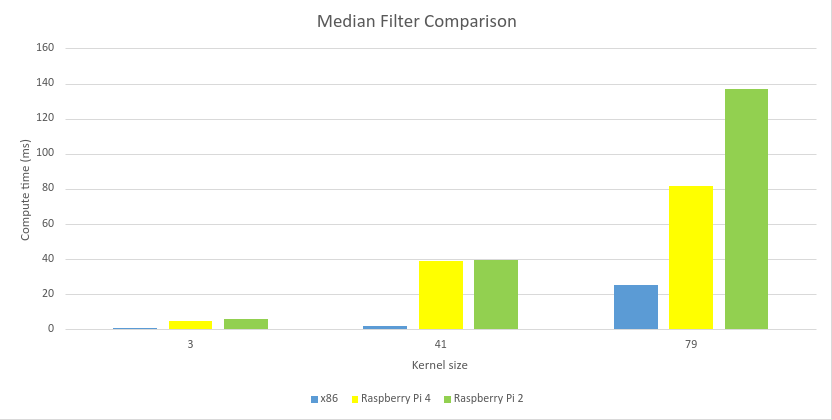
\includegraphics[width=0.8\textwidth, height=0.5\textwidth]{resources/Measurements_Median.png}}
    \caption{Performance comparison on Median filter results}
\end{figure}

As shown in \cref{fig:medianResults}, all three systems are on par for lower computational sizes, however, as
the workload increases, compute times increase exponentially, due to the required calculation increasing with
the square of the kernel size. With the x86 outperforming both ARM platforms, as was expected from the 
technical specifications, it can be noted that the Raspberry Pi systems give similar results when working
on medium workloads, with the Raspberry Pi 2 falling behind only when the computational requirements are
significantly increased.

Another relevant metric is the time in which the directional Sobel filter is computed on all three platforms,
with it being one of the more visually impactful operations available.

\begin{figure}[H]
    \label{fig:sobelResults}
    \frame{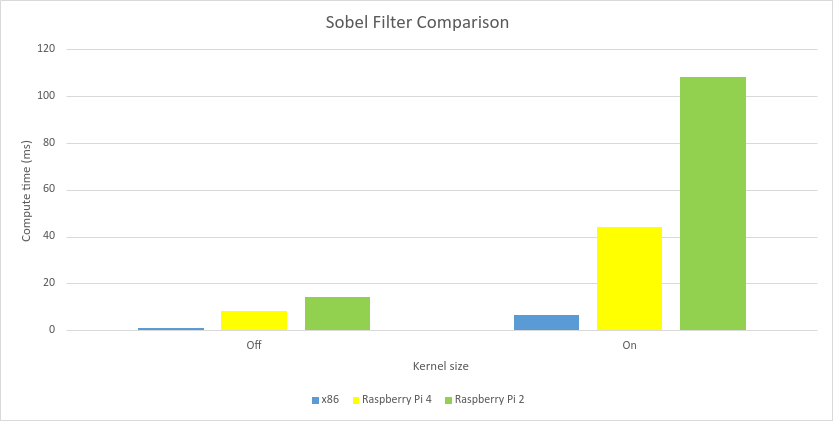
\includegraphics[width=0.8\textwidth, height=0.5\textwidth]{resources/Measurements_Sobel.png}}
    \caption{Performance comparison on Sobel filter results}
\end{figure}

It can be observed in \cref{fig:sobelResults} that only the x86 can perform the necessary trigonometric 
computations within the required time limit of \(33ms\), with both Raspberry Pi systems experiencing frame
drops.

Although the x86 is the decisive leader in terms of computational prowess, other factors such as touchsecrren
capability, setup requirements, visual impact and cost have to be considered when choosing the optimal system
for the demonstration.

